% Festlegung des Allgemeinen Dokumentenformats
\documentclass[a4paper,12pt,headsepline]{scrartcl}

% Umlaute unter UTF8 nutzen
\usepackage[utf8]{inputenc}

% Variablen
%Variablen welche innerhalb der gesamten Arbeit zur Verfügung stehen sollen
\newcommand{\titleDocument}{Bachelorarbeit}
\newcommand{\subjectDocument}{
    Analyse der Echtzeitfähigkeit von Micro-ROS und FreeRTOS am Beispiel einer
    Robotersteuerungssoftware
}


% weitere Pakete
% Grafiken aus PNG Dateien einbinden
\usepackage{graphicx}
\usepackage{tikz}

% Deutsche Sonderzeichen und Silbentrennung nutzen
\usepackage[ngerman]{babel}

% Eurozeichen einbinden
\usepackage[right]{eurosym}

% Zeichenencoding
\usepackage[T1]{fontenc}

\usepackage{lmodern}

% floatende Bilder ermöglichen
%\usepackage{floatflt}

% mehrseitige Tabellen ermöglichen
\usepackage{longtable}

% Unterstützung für Schriftarten
%\newcommand{\changefont}[3]{ 
%\fontfamily{#1} \fontseries{#2} \fontshape{#3} \selectfont}

% Packet für Seitenrandabständex und Einstellung für Seitenränder
\usepackage{geometry}
\geometry{left=3.5cm, right=2.5cm, top=3cm, bottom=2.5cm}

% Paket für Boxen im Text
\usepackage{fancybox}

% bricht lange URLs "schön" um
\usepackage[hyphens,obeyspaces,spaces]{url}

% Paket für Textfarben
\usepackage{color}

% Mathematische Symbole importieren
\usepackage{amssymb}

\usepackage{amsmath}

% auf jeder Seite eine Überschrift (alt, zentriert)
%\pagestyle{headings}

\usepackage{pdfpages}

% erzeugt Inhaltsverzeichnis mit Querverweisen zu den Abschnitten (PDF Version)
\usepackage[bookmarksnumbered,pdftitle={\titleDocument},hyperfootnotes=false]{hyperref}
%\hypersetup{colorlinks, citecolor=red, linkcolor=blue, urlcolor=black}
%\hypersetup{colorlinks, citecolor=black, linkcolor= black, urlcolor=black}

% neue Kopfzeilen mit fancypaket
\usepackage{fancyhdr} %Paket laden
\pagestyle{fancy} %eigener Seitenstil
\fancyhf{} %alle Kopf- und Fußzeilenfelder bereinigen
\fancyhead[L]{\nouppercase{\leftmark}} %Kopfzeile links
\fancyhead[C]{} %zentrierte Kopfzeile
\fancyhead[R]{\thepage} %Kopfzeile rechts
\renewcommand{\headrulewidth}{0.4pt} %obere Trennlinie
%\fancyfoot[C]{\thepage} %Seitennummer
%\renewcommand{\footrulewidth}{0.4pt} %untere Trennlinie

% change font to serif for headings - buggy
% \usepackage{sectsty}
% \allsectionsfont{\normalfont\bfseries}

% für Tabellen
\usepackage{array}

% Runde Klammern für Zitate
%\usepackage[numbers,round]{natbib}

% Festlegung Art der Zitierung - Havardmethode: Abkuerzung Autor + Jahr
\bibliographystyle{alphadin}

% Schaltet den zusätzlichen Zwischenraum ab, den LaTeX normalerweise nach einem Satzzeichen einfügt.
%\frenchspacing

% Paket für Zeilenabstand
\usepackage{setspace}

% für Bildbezeichner
\usepackage{capt-of}

% für Stichwortverzeichnis
\usepackage{makeidx}

%Konfiguriere das Inhaltsverzeichnis
\usepackage{tocbasic}
\DeclareTOCStyleEntries[
  raggedentrytext,
  numwidth=0pt,
  numsep=1ex,
  dynnumwidth,
]{tocline}{chapter,section,subsection,subsubsection,paragraph,subparagraph}
\DeclareTOCStyleEntries[
  indent=0pt,
  linefill=\TOCLineLeaderFill,
]{tocline}{section,subsection,subsubsection,paragraph,subparagraph}


% für Listings
% \usepackage{listings}
% \lstset{numbers=left, numberstyle=\tiny, numbersep=5pt, keywordstyle=\color{black}\bfseries, stringstyle=\ttfamily,showstringspaces=false,basicstyle=\footnotesize,captionpos=b}
\usepackage{xcolor}
\usepackage[newfloat]{minted}
\usepackage{caption}
\usepackage{fancyhdr}
\newenvironment{code}{\captionsetup{type=listing}}{}
\SetupFloatingEnvironment{listing}{name=Quellcode}
\setminted{
    linenos,
	frame=single,
    bgcolor=black!5,
    fontsize=\footnotesize
}
\usepackage{graphicx}  % Add this to your preamble

\usepackage[withpage]{acronym}

% Absatz ohne Einrückung
\setlength{\parskip}{1em} % 1em entspricht der Breite eines 'M'-Zeichens
\setlength{\parindent}{0pt}

% Indexerstellung
\makeindex

% Abkürzungsverzeichnis
\usepackage[german]{nomencl}
\let\abbrev\nomenclature

% Abkürzungsverzeichnis LiveTex Version
% Titel des Abkürzungsverzeichnisses
\renewcommand{\nomname}{Abkürzungsverzeichnis}
% Abstand zwischen Abkürzung und Erläuterung
\setlength{\nomlabelwidth}{.25\textwidth}
% Zwischenraum zwischen Abkürzung und Erläuterung mit Punkten
\renewcommand{\nomlabel}[1]{#1 \dotfill}
% Variation des Abstandes der einzelnen Abkürzungen zu einander
\setlength{\nomitemsep}{-\parsep}
% Index mit Abkürzungen erzeugen
\makenomenclature
%\makeglossary

% Abkürzungsverzeichnis TeTEX Version
% \usepackage[german]{nomencl}
% \makenomenclature
% %\makeglossary
% \renewcommand{\nomname}{Abkürzungsverzeichnis}
% \AtBeginDocument{\setlength{\nomlabelwidth}{.25\columnwidth}}
% \renewcommand{\nomlabel}[1]{#1 \dotfill}
% \setlength{\nomitemsep}{-\parsep}

% Optional: Einzelne Zeilen am Anfang einer Seite unterdrücken (Schusterjungen)
% \clubpenalty = 10000
% Optional: Einzelne Zeilen am Ende einer Seite unterdrücken (Hurenkinder)
% \widowpenalty = 10000
% \displaywidowpenalty = 10000

\begin{document}
% hier werden die Trennvorschläge inkludiert
%hier müssen alle Wörter rein, welche Latex von sich auch nicht korrekt trennt bzw. bei denen man die genaue Trennung vorgeben möchte
\hyphenation{
Film-pro-du-zen-ten
Lux-em-burg
Soft-ware-bau-steins
zeit-in-ten-siv
}


% Schriftart Helvetica verwenden
%\usepackage{helvet}
%\renewcommand\familydefault{\sfdefault}

% Leere Seite am Anfang
%\thispagestyle{empty} % erzeugt Seite ohne Kopf- / Fusszeile
%\mbox{}
%\newpage

% Titelseite %
\thispagestyle{empty}

% % Logo
% \begin{figure}[t]
%  \centering
%  
\includegraphics[width=0.3\textwidth]{assets/fhlogo.pdf}
% \end{figure}

\begin{center}
\textbf{\Large{~\titleDocument}}
\end{center}
\begin{verbatim}





\end{verbatim}
\begin{center}
\doublespacing
\textbf{\LARGE{\subjectDocument}}\\
\singlespacing
\end{center}
\begin{verbatim}
















\end{verbatim}
\begin{center}
\textbf{
    An der Fachhochschule Dortmund \\
    im Fachbereich Informatik \\
    Studiengang Technische Informatik \\
    erstellte Thesis \\
    zur Erlangung des akademischen Grades \\
    Bachelor of Science \\
    B. Sc. \\
}
\end{center}
\begin{center}
    \textbf{Xu, Zijian \linebreak
    geboren am 25.09.1998 \linebreak
    7204211
    }
\end{center}
\begin{flushleft}
\begin{tabular}{llll}
\textbf{Betreuung durch:} & & Prof. Dr. Christof Röhrig &\\
    & & M. Sc. Alexander Miller &\\
\textbf{Version vom:} & & Dortmund, \today &\\
\end{tabular}
\end{flushleft}


% römische Numerierung
\pagenumbering{roman}

% 1.5 facher Zeilenabstand
\onehalfspacing

\newpage

% Einleitung / Abstract
\thispagestyle{empty}
\section*{Kurzfassung}

Diese Arbeit analysiert die Echtzeitfähigkeit von Micro-ROS und FreeRTOS anhand
einer Robotersteuerungssoftware. Ziel ist der Vergleich beider Systeme
hinsichtlich ihres Echtzeitverhaltens mit Schwerpunkt auf den Ausführungszeiten.
Dazu wird zunächst die bestehende Micro-ROS-Steuerungssoftware auf FreeRTOS
portiert. Anschließend wird eine zyklengenaue Messmethode für den Programmlauf
basierend auf der Data Watchpoint and Trace Unit (DWT) der ARM-Architektur
entwickelt. Zum Abschluss werden die Laufzeitdaten visualisiert und ausgewertet.
Die Ergebnisse verdeutlichen die unterschiedlichen Schwerpunkte beider
Plattformen: Micro-ROS punktet durch die Kompatibilität mit dem ROS-Ökosystem,
während FreeRTOS mit minimalen Latenzen und deterministischem Scheduling
deutlich besseres Echtzeitverhalten bietet. Die Analyse bestätigt zudem den
maßgeblichen Einfluss der Cache-Nutzung auf die Rechenleistung.

\section*{Abstract}

This thesis analyzes the real-time capabilities of micro-ROS and FreeRTOS using
a robotic control software. The goal is to compare both systems regarding their
real-time behavior emphasized on the execution times. First, the existing
micro-ROS control software is ported to FreeRTOS. Next, a cycle-accurate
measurement method for program execution based on ARM's Data Watchpoint and
Trace Unit (DWT)is developed. Finally, the runtime data is evaluated. The
evaluation of the results highlights the different strengths of both platforms:
micro-ROS stands out due to its compatibility with the ROS ecosystem, while
FreeRTOS achieves superior real-time behavior through minimal latencies and
deterministic scheduling. Additionally, the analysis confirms the significant
impact of the cache utilization on system performance.


% einfacher Zeilenabstand
\singlespacing

\newpage
% Seitenzählung bei Inhaltsverzeichnis beginnen
\setcounter{page}{1}

% Inhaltsverzeichnis anzeigen
\thispagestyle{empty}
\tableofcontents

\newpage
% das Abbildungsverzeichnis
% Verion 1: Abbildungsverzeichnis MIT führender Nummberierung endgueltig anzeigen
\listoffigures
% Abbildungsverzeichnis soll im Inhaltsverzeichnis auftauchen
\addcontentsline{toc}{section}{Abbildungsverzeichnis}

% Verion 2: Abbildungsverzeichnis OHNE führende Nummberierung endgueltig anzeigen
%\begingroup
%\renewcommand\numberline[1]{}
%\listoffigures
%\endgroup


% % das Tabellenverzeichnis
% \newpage
% % \fancyhead[L]{Abbildungsverzeichnis / Abkürzungsverzeichnis} %Kopfzeile links
% % Tabellenverzeichnis endgültig anzeigen
% \listoftables
% % Tabellenverzeichnis soll im Inhaltsverzeichnis auftauchen
% \addcontentsline{toc}{section}{Tabellenverzeichnis}

% das Quellcodeverzeichnis
\newpage
\renewcommand*{\listlistingname}{Quellcodeverzeichnis}
\listoflistings % Add Quellcodeverzeichnis
\addcontentsline{toc}{section}{Quellcodeverzeichnis}

% das Abkürzungsverzeichnis
\newpage
% das Abkürzungsverzeichnis ausgeben
\fancyhead[L]{Abkürzungsverzeichnis} %Kopfzeile links
\section*{Abkürzungsverzeichnis}

\begin{acronym}
\end{acronym}

% \printnomenclature[3cm]
% Abkürzungsverzeichnis soll im Inhaltsverzeichnis auftauchen
\addcontentsline{toc}{section}{Abkürzungsverzeichnis}


%%%%%%% EINLEITUNG %%%%%%%%%%%%
\newpage
\fancyhead[L]{\nouppercase{\leftmark}} %Kopfzeile links

% 1,5 facher Zeilenabstand
\onehalfspacing

% arabische Seitennummerierung ab hier
\pagenumbering{arabic}

% Alternative Einbindung des Abstract in Kapitel "0" falls gewünscht
%\setcounter{section}{-1}
%\setcounter{page}{0}

% Option: Einbindung abstract
%\section*{Kurzfassung}

Diese Arbeit analysiert die Echtzeitfähigkeit von Micro-ROS und FreeRTOS anhand
einer Robotersteuerungssoftware. Ziel ist der Vergleich beider Systeme
hinsichtlich ihres Echtzeitverhaltens mit Schwerpunkt auf den Ausführungszeiten.
Dazu wird zunächst die bestehende Micro-ROS-Steuerungssoftware auf FreeRTOS
portiert. Anschließend wird eine zyklengenaue Messmethode für den Programmlauf
basierend auf der Data Watchpoint and Trace Unit (DWT) der ARM-Architektur
entwickelt. Zum Abschluss werden die Laufzeitdaten visualisiert und ausgewertet.
Die Ergebnisse verdeutlichen die unterschiedlichen Schwerpunkte beider
Plattformen: Micro-ROS punktet durch die Kompatibilität mit dem ROS-Ökosystem,
während FreeRTOS mit minimalen Latenzen und deterministischem Scheduling
deutlich besseres Echtzeitverhalten bietet. Die Analyse bestätigt zudem den
maßgeblichen Einfluss der Cache-Nutzung auf die Rechenleistung.

\section*{Abstract}

This thesis analyzes the real-time capabilities of micro-ROS and FreeRTOS using
a robotic control software. The goal is to compare both systems regarding their
real-time behavior emphasized on the execution times. First, the existing
micro-ROS control software is ported to FreeRTOS. Next, a cycle-accurate
measurement method for program execution based on ARM's Data Watchpoint and
Trace Unit (DWT)is developed. Finally, the runtime data is evaluated. The
evaluation of the results highlights the different strengths of both platforms:
micro-ROS stands out due to its compatibility with the ROS ecosystem, while
FreeRTOS achieves superior real-time behavior through minimal latencies and
deterministic scheduling. Additionally, the analysis confirms the significant
impact of the cache utilization on system performance.

%\newpage

% einzelne Kapitel werden hier eingebunden
\section{Einleitung}

Die vorliegende Bachelorarbeit hat zunächst als Ziel, die bestehende
Robotersteuerungssoftware von Micro-ROS auf FreeRTOS zu portieren, um die
Echtzeitleistung beider Plattformen miteinander zu vergleichen.

Beide Systeme sind für die PID-geregelte Steuerung eines mobilen Roboters auf
einem Cortex-M7 Mikrocontroller ausgelegt, unterscheiden sich aber in ihrer
zugrundeliegenden Softwarearchitektur: Während Micro-ROS auf dem \ac{ROS 2}
Framework aufbaut und somit eine höhere Abstraktionsebene durch eine
standardisierte Kommunikationsschnittstelle in Form einer integrierten
\ac{DDS}-Middleware bietet, basiert dies selbst auf einem \ac{RTOS} wie FreeRTOS
(\ref{fig:micro_ros_arch}). Die Portierung kann daher als eine Reduzierung von
Abhängigkeiten betrachtet werden. Dies ermöglicht eine direktere und damit
effizientere Nutzung der zugrundeliegenden Echtzeit- sowie Speicherressourcen.

\begin{figure}[htb] \centering
    \includegraphics[width=0.8\textwidth]{assets/Micro-ROS_architecture}
    \caption{Micro-ROS Architektur\cite[S. 6]{koubaa2023}}
    \label{fig:micro_ros_arch}
\end{figure}

Daher wird die Steuerungssoftware erneut auf Basis von FreeRTOS implementiert,
um demnach die Echtzeitleistung auf beiden Plattformen zu analysieren und zu
vergleichen. Die Analyse soll unter anderem aufzeigen, inwiefern FreeRTOS durch
die Eliminierung dieser zusätzlichen Abhängigkeit eine effizientere und
leichtgewichtigere Lösung darstellt. Dabei soll der Einsatz einer zyklengenauen
Messung des Programmablaufs ermöglicht werden, um fundierte Aussagen über das
Echtzeitverhalten beider Systeme zu treffen und den Leistungsgewinn quantitativ
zu belegen.

Die Arbeit gliedert sich in vier Teile: Nach der Einführung in die grundlegenden
Konzepte wird zunächst die Implementierung der Steuerungssoftware auf FreeRTOS
beschrieben. Anschließend wird die Implementierung zur Erfassung von
Laufzeitdaten detailliert gezeigt. Den Abschluss bildet die quantitative
Präsentation der Ergebnisse, deren Bewertung sowie mögliche Optimierungsansätze.

\newpage

\section{Hintergrund}

Die vorliegende Bachelorarbeit hat zum Ziel, die Robotersteuerungssoftware, die
derzeit auf Micro-ROS basiert, auf FreeRTOS zu portieren, um einen
vergleichenden Leistungsanalyse zwischen beiden Plattformen durchzuführen. Beide
Systeme sind für die Steuerung eines mobilen Roboters auf einem Cortex-M7
Mikrocontroller von Arm konzipiert, unterscheiden sich jedoch in ihrer
grundlegenden Architektur, was sich auch in ihrer Echtzeitfähigkeit und
Ressourcennutzung widerspiegelt. Während Micro-ROS auf der \ac{ROS 2} aufbaut
und eine höhere Abstraktionsebene sowie standardisierte
Kommunikationsschnittstellen mittels der \ac{DDS}-Middleware bietet, basiert
Micro-ROS selbst auf FreeRTOS. Die Portierung der Robotersteuerungssoftware von
Micro-ROS auf FreeRTOS kann daher als eine Reduzierung der Abhängigkeitsebene
betrachtet werden. Dies ermöglicht eine direktere und effizientere Nutzung der
zugrunde liegenden Echtzeit-, sowie Speicherressourcen.

\begin{figure}[htb] \centering
    \includegraphics[width=0.8\textwidth]{assets/Micro-ROS_architecture}
    \caption{Micro-ROS Architektur\cite[S. 6]{koubaa2023}}
    % \label{fig:uros_architecture}
\end{figure}

Nach dem Wechsel zu FreeRTOS wird die Echtzeitleistung der Steuerungssoftware
analysiert mit einem besonderen Fokus auf den Overhead, der durch die
Micro-ROS-Schicht verursacht wird. Der Vergleich soll aufzeigen, inwiefern
FreeRTOS durch die Eliminierung dieser zusätzlichen Abhängigkeit eine
effizientere und leichtgewichtige Lösung für kritische Roboteranwendungen
darstellt. Dabei soll der Einsatz einer zyklengenaue Messung des Programmablaufs
ermöglichen, fundierte Aussagen über die Echtzeitfähigkeit beider Plattformen zu
treffen, und den Leistungsgewinn anhand von diesem Beispiel für eine
Steuerungssoftware quantitativ zu belegen.

\subsection{FreeRTOS}

FreeRTOS ist ein Open-Source, leichtgewichtiges \ac{RTOS}, das speziell für
eingebettete Systeme entwickelt wurde. Es zeichnet sich unter anderem durch
deterministisches Verhalten mit Echtzeitgarantie sowie Konfigurierbarkeit der
Heap-Allokation aus. Diese Eigenschaften machen es zu einer geeigneten Wahl für
Robotersteuerungssoftware, insbesondere wenn Echtzeitanforderungen und
effiziente Ressourcennutzung im Vordergrund stehen.

\subsubsection{Konzepte}

FreeRTOS unterscheidet sich von der Bare-Metal-Programmierung dadurch, dass es
eine nützliche Abstraktionsebene für den Nutzer bereitstellt. Diese
Abstraktionen ermöglichen es, komplexere Echtzeitanforderungen zu bewältigen,
ohne dass der Nutzer diese Funktionalitäten selbst implementieren muss.
Beispiele hierfür sind Timer mit konfigurierbarer Genauigkeit (basierend auf den
sogenannten Tick \cite{freertos_rtos_tick, freertos_tick_resolution}),
threadsichere Queues sowie Semaphore und Mutexe \cite{freertos_queues}. Diese
Komponenten bieten fertige Lösungen für häufige Herausforderungen in der
Entwicklung eingebetteter Systeme, sodass der Nutzer solche Werkzeuge nicht mehr
selbst anfertigen muss.

Im Fokus dieser Arbeit stehen Queues und „Direct Task Notifications“, die in der
Robotersteuerungssoftware zum Einsatz kommen, sowie Semaphore und die
sogenannten „Trace Hooks” für die darauffolgende Echtzeitanalyse. Diese
Komponenten werden im Folgenden detailliert erläutert.

\paragraph{Queues}

Queues sind eine der Kernkomponenten von FreeRTOS und dienen der
Interprozesskommunikation zwischen Tasks. Sie ermöglichen den threadsicheren
Austausch von Daten, und können sowohl zur Datenübertragung als auch zur
Synchronisation von Tasks verwendet werden, da dedizierte
(Ressourcen-)\\Synchronisationsmechanismen wie Semaphore und Mutexe sind auf
Queues aufgebaut \cite{freertos_semphr_incl}.

\paragraph{Semaphore}

Wie bereits kurz erwähnt, sind Semaphore und Mutexe Tools, die den Zugriff auf
gemeinsame Ressourcen koordinieren, wobei Semaphore auch zur Synchronisation von
Tasks genutzt werden können. Semaphoren sind einfache Mechanismen ohne
Unterstützung von Prioritätsvererbung, bei der eine Task mit Besitz von einem
\textit{Mutex} mit einer niedrigeren Priorität künstlich auf die gleiche
Priorität der auf den Mutex wartenden Task angehoben
wird~\cite{wikipedia_priority_inheritance}. Wenn eine Ressource dann nur mit
einem Semaphor geschützt ist, kann dies zu Prioritätsinversion führen, bei der
eine höher priorisierte Task aufgrund einer blockierten gemeinsam genutzten
Ressource nicht ausgeführt werden kann, sodass der Scheduler stattdessen eine
niedriger priorisierte Task auswählen muss, bis die Ressource freigegeben ist.
\cite{wikipedia_priority_inversion}.

\begin{figure}[htb]
    \centering
    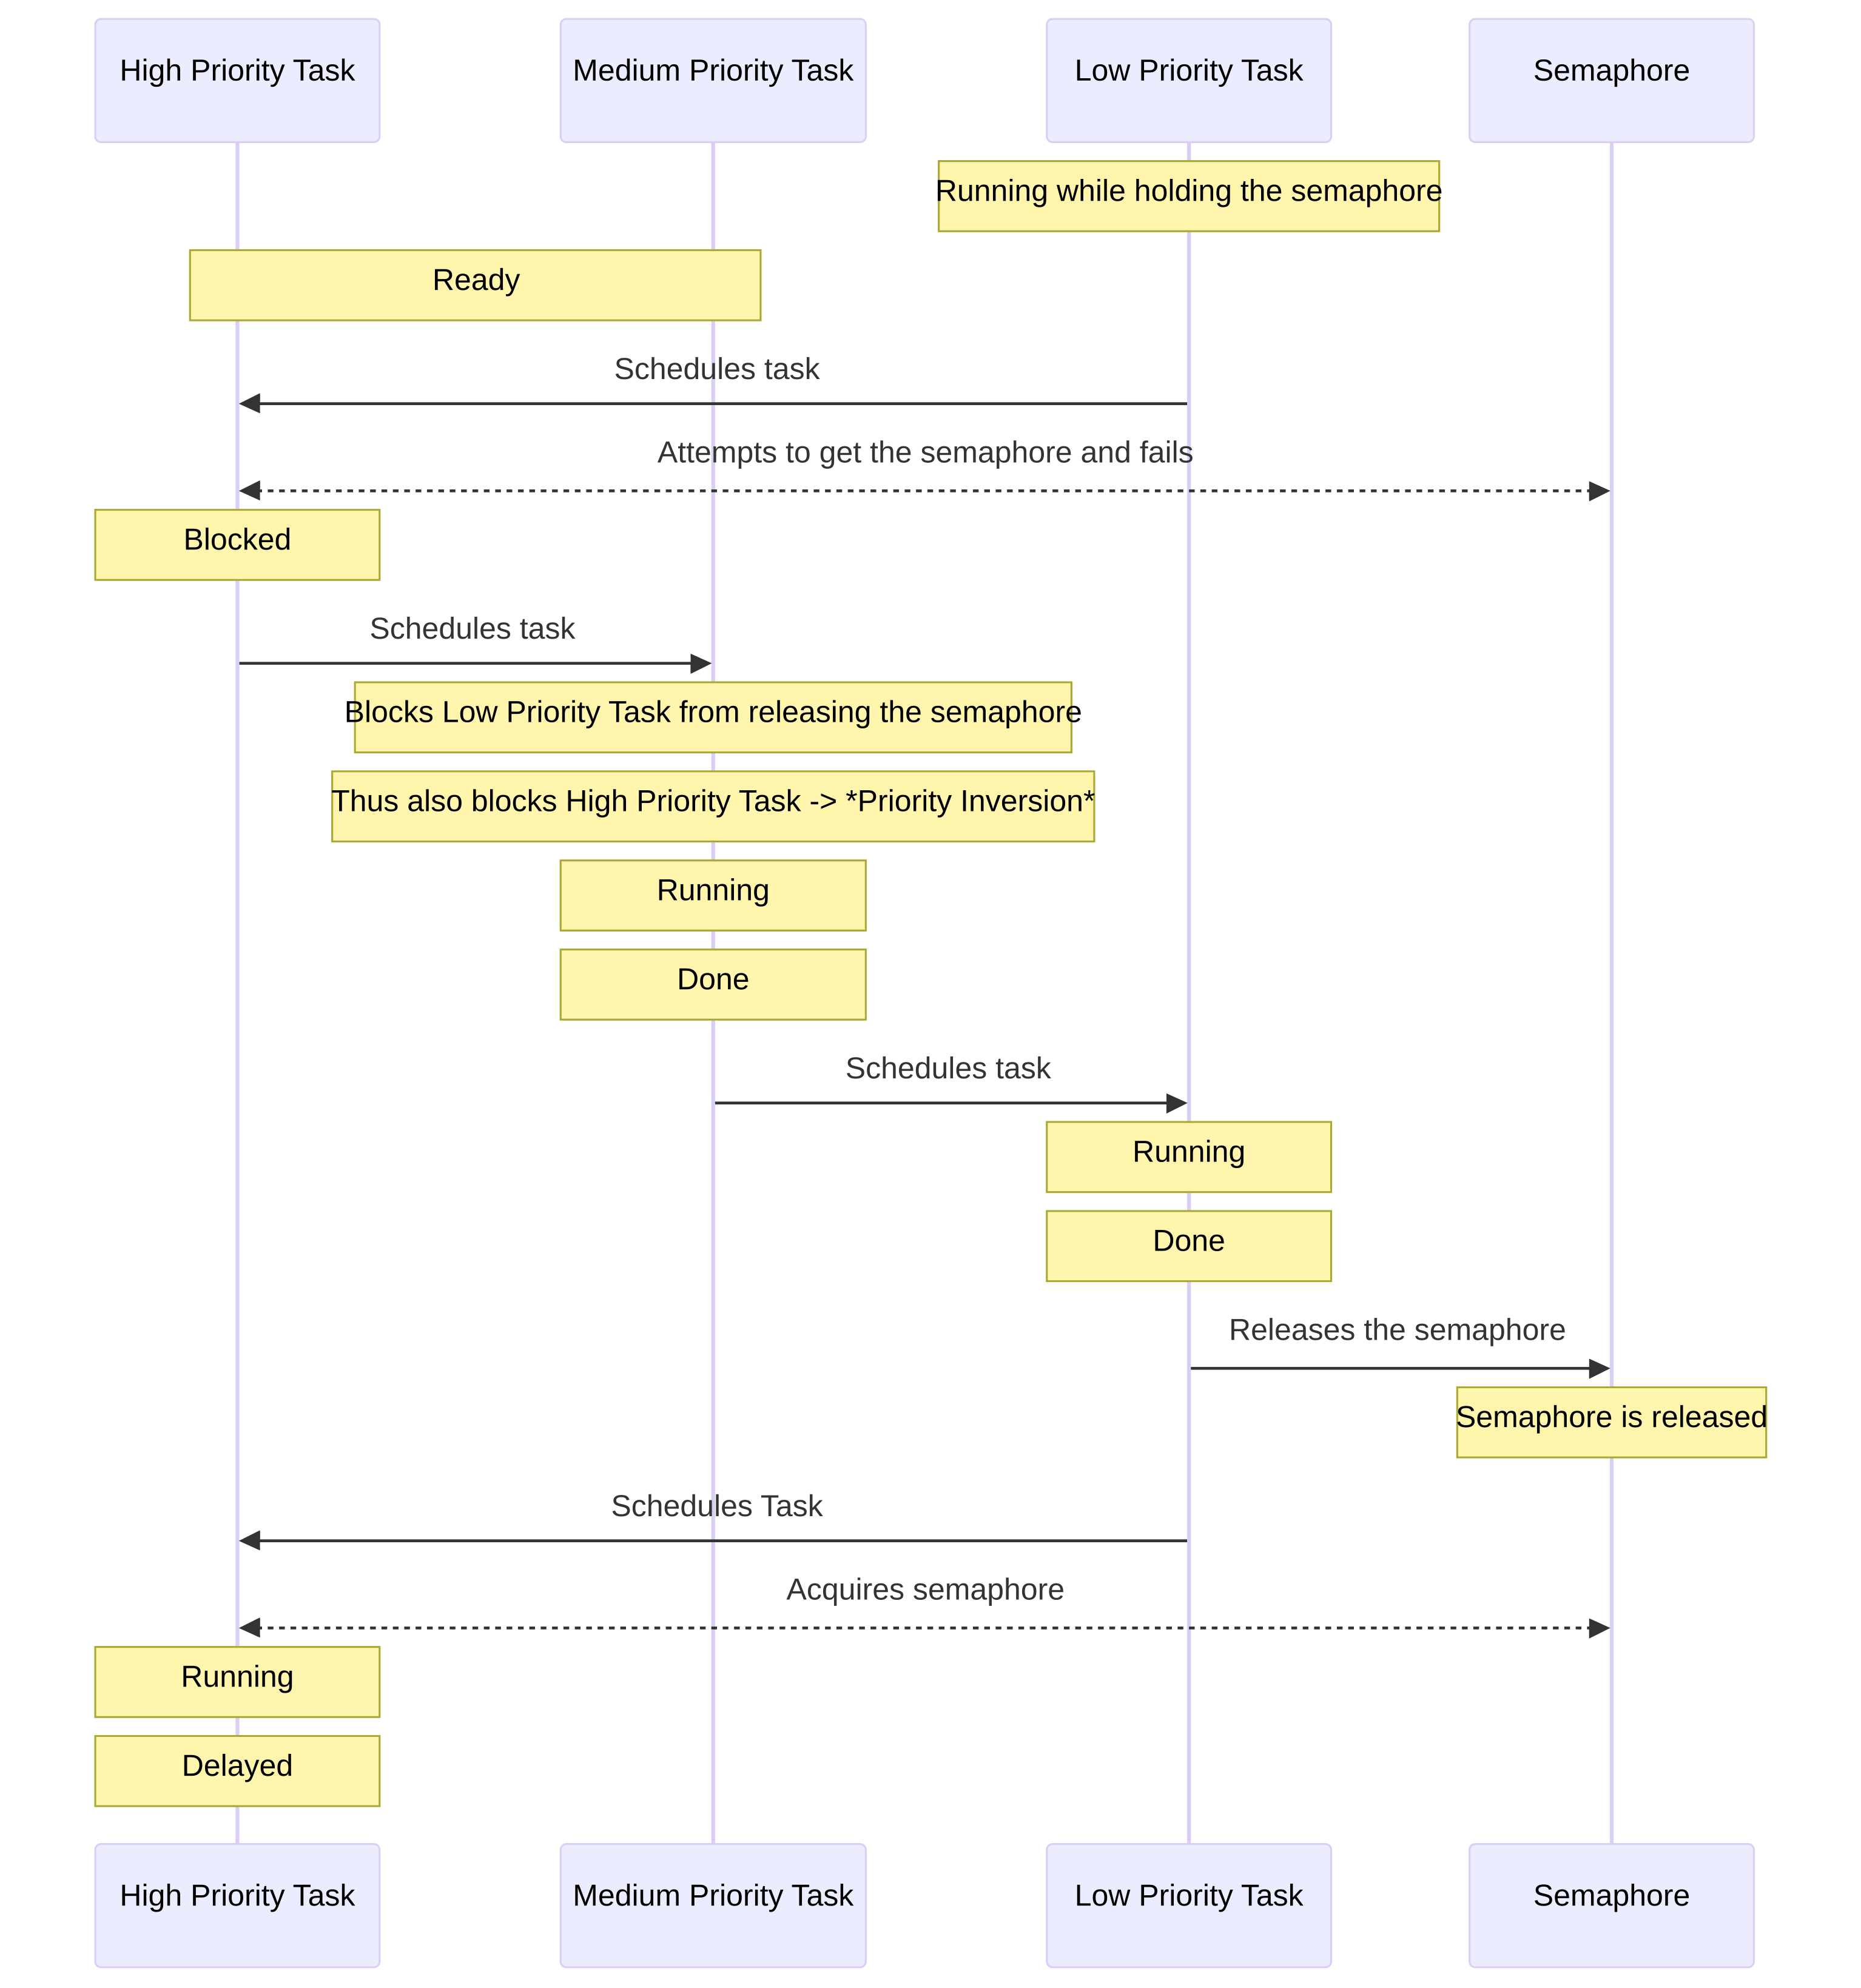
\includegraphics[width=1\textwidth]{assets/prio_inversion}
    \caption{Prioritätsinversion}
\end{figure}

\paragraph{Mutexe} \label{sec:mutex}

Im Gegensatz dazu sind Mutexe (Mutual Exclusion) Synchronisationsmechanismen,
die Prioritätsvererbung implementieren \cite{freertos_mutexes}. Wenn eine Task
auf einen Mutex wartet, der von einer niedriger priorisierten Task gehalten
wird, wird diese Task temporär auf die Priorität der wartenden Task
erhöht~\cite{FreertosForumSemphMtx}, so dass er den Mutex und damit die von der
watenden Task benötigte Ressource so schnell wie möglich wieder freigeben kann.

\begin{figure}[htb]
    \centering
    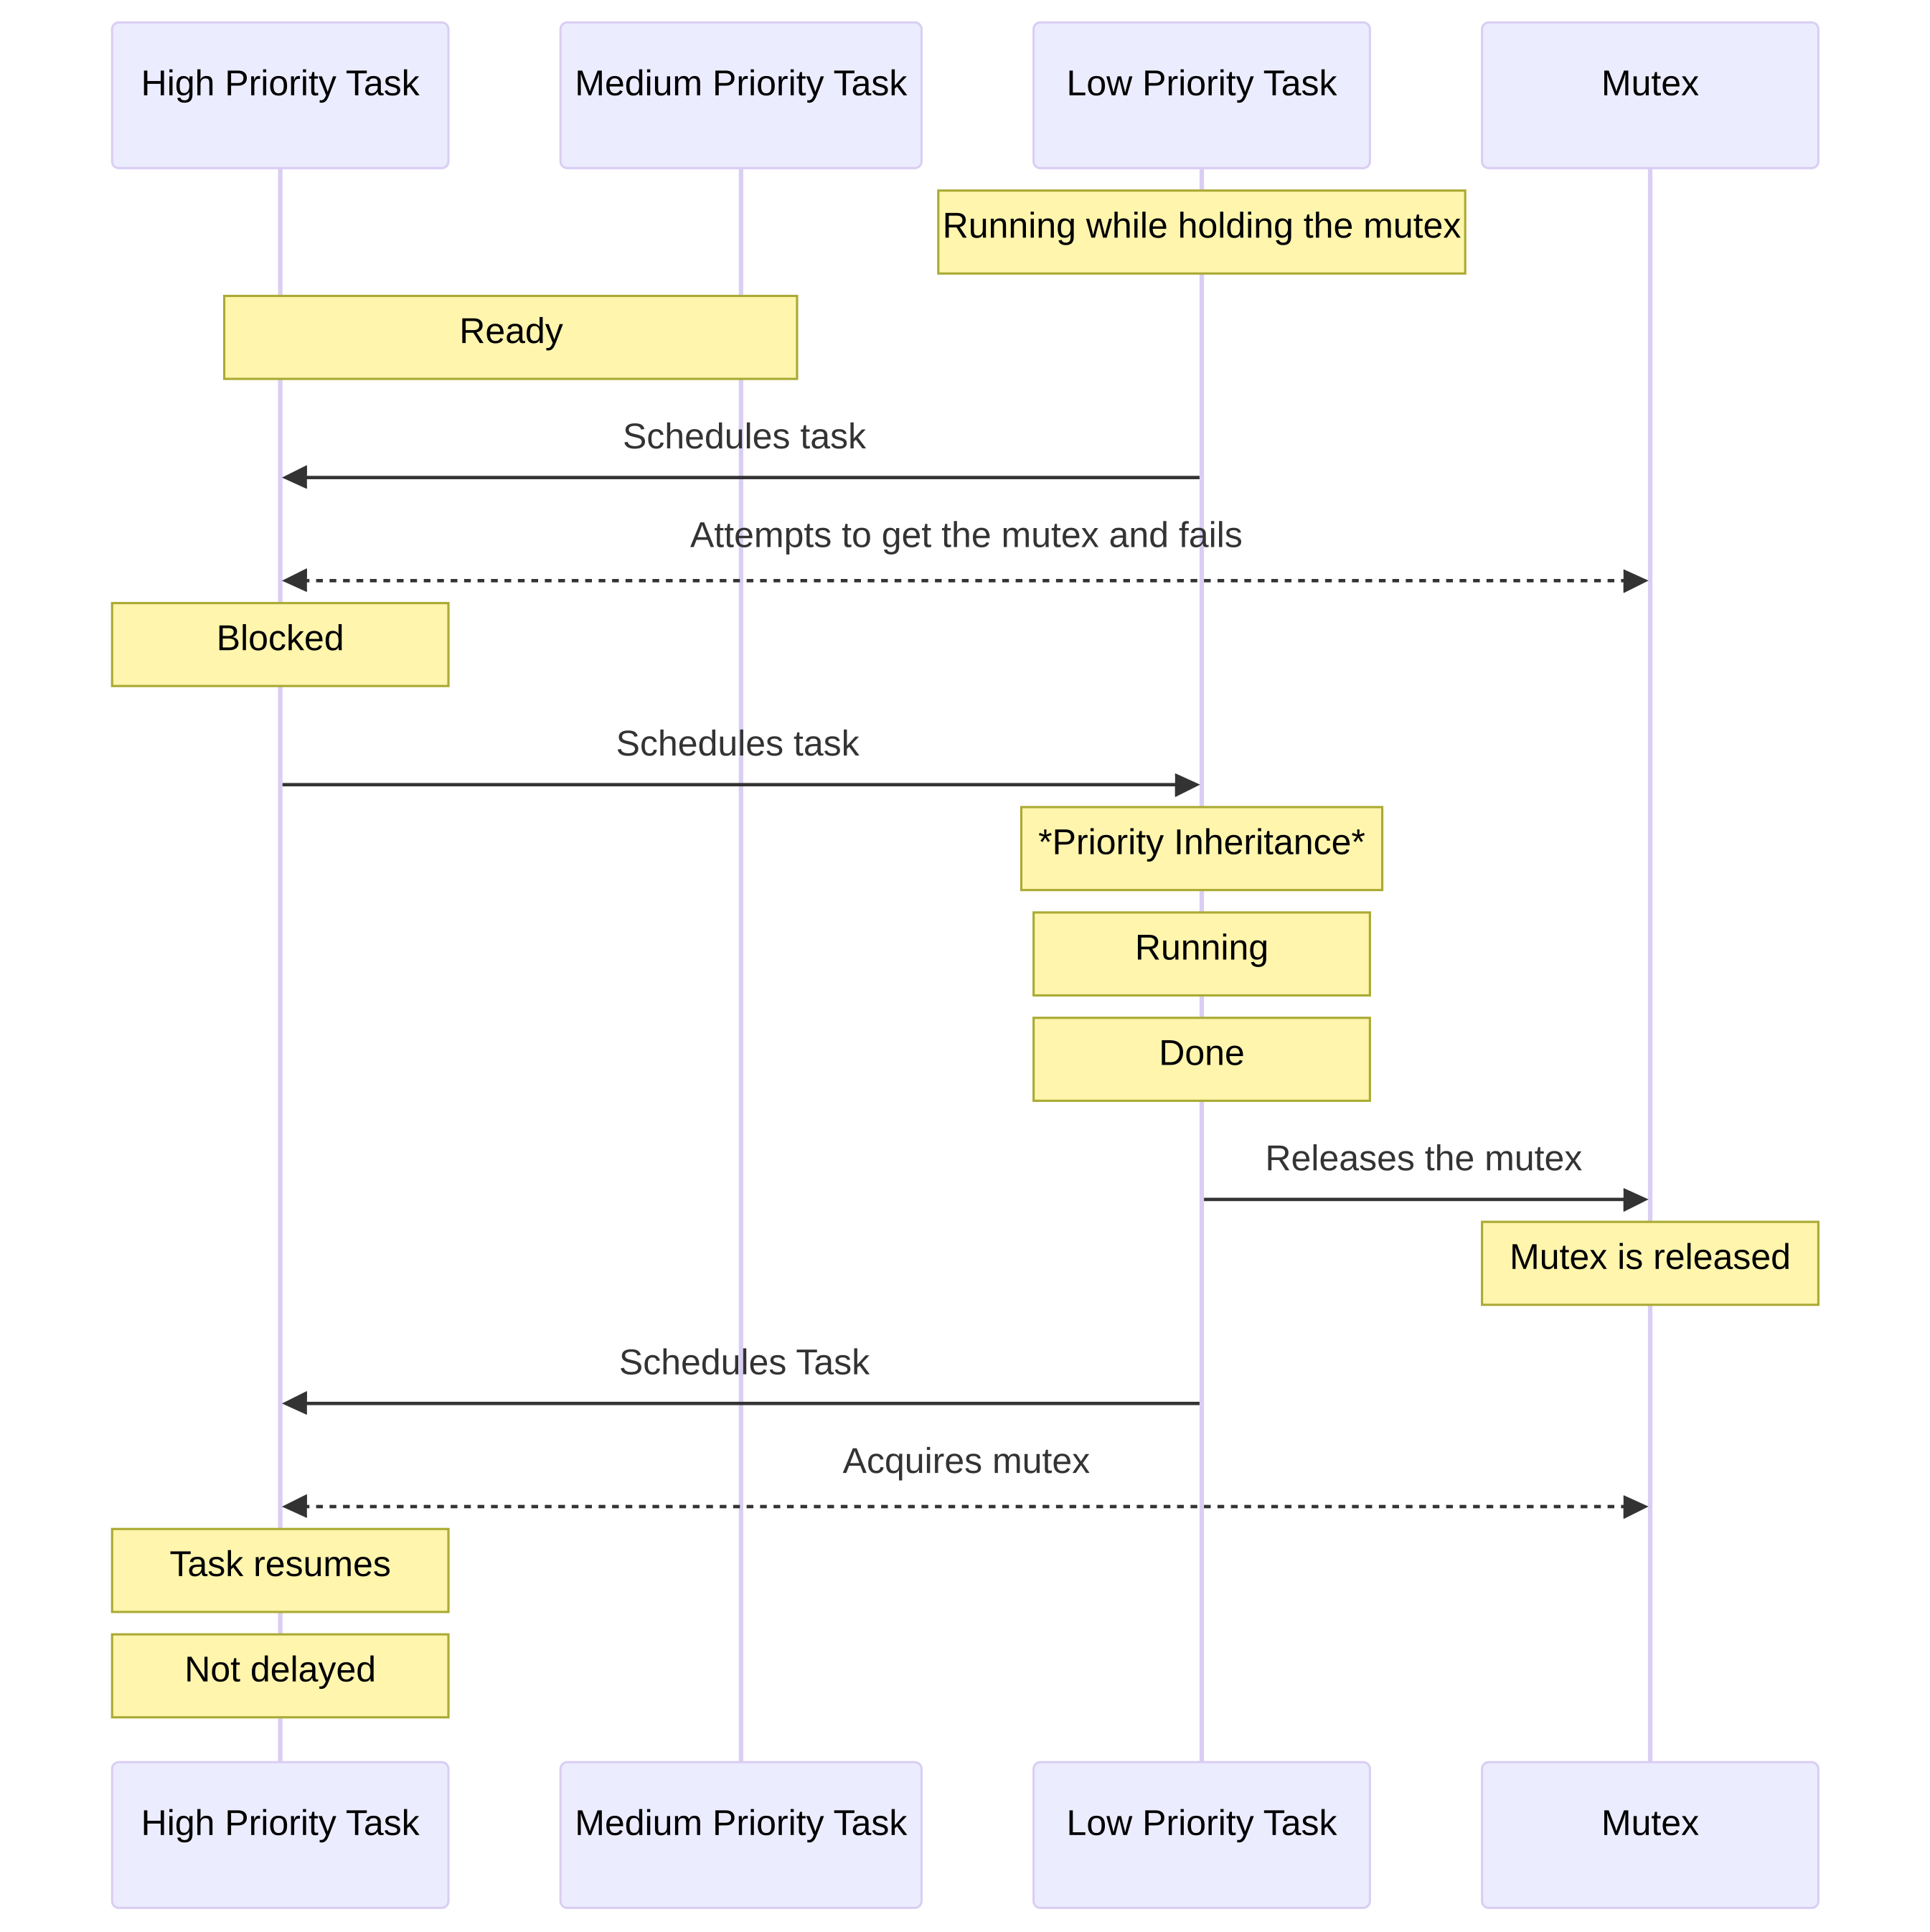
\includegraphics[width=1\textwidth]{assets/prio_inheritance}
    \caption{Prioritätsvererbung}
\end{figure}

\paragraph{Direct Task Notifications} \label{sec:direct_task_notification}

Direct Task Notifications sind ein effizienterer und ressourcenschonenderer
Mechanismus zur Task-Synchronisation \cite{freertos_task_notifications_desc}. Im
Gegensatz zu Semaphoren senden sie direkte Signale an eine Task, ohne die
zugrunde liegenden Queues zu benötigen, indem sie einfach einen internen Zähler
einer Task verändern \cite{freertos_tasks_c_308}. Analog zu Semaphoren wird
mittels Funktionen wie zum Beispiel \mintinline{c}|ulTaskNotifyGive()| dieser
Zähler inkrementiert~\cite{freertos_tasks_c_4990}, während Funktionen wie
\mintinline{c}|ulTaskNotifyTake()| ihn wieder
dekrementieren~\cite{freertos_tasks_c_4614}. Das Entblocken einer Task mittels
Direct Task Notifications soll bis zu 45\% schneller sein und benötigt weniger
RAM \cite{freertos_task_notifications_usage}.

\paragraph{Trace Hooks} \label{sec:trace_hooks}

„Trace Hooks“ sind spezielle Mackos von der FreeRTOS-API, deren Nutzung es
beispielsweise ermöglicht, Ereignisse im System zu verfolgen und zu
protokollieren. Diese Makros werden innerhalb von Interrupts beim Schedulen
aufgerufen und sollten immer vor der Einbindung von
\mintinline{text}|FreeRTOS.h| definiert werden \cite{freertos_rtos_trace_hooks}.

\subsection{Nutzung von Caches}

Caches sind schnelle Speicherkomponenten, die dazu dienen, Zugriffe auf häufig
verwendete Daten und Befehle zu beschleunigen und den Energieverbrauch zu
reduzieren \cite{ka001150}. In vielen modernen Mikrocontrollern, wie dem
Cortex-M7, ist der L1-Cache (Level 1 Cache) jeweils in einen Datencache
(D-Cache) und einen Instruktionscache (I-Cache) unterteilt \cite[S. 6]{an4667}.
Da der Zugriff auf den Hauptspeicher sowie auf den Flash generell viel langsamer
ist und mehrere Taktzyklen dauert~\cite{stm32_memory_sections}, kann mit
L1-Caches Null-Waitstate ermöglicht werden~\cite[S. 6]{an4667}, wodurch der
Prozessor ohne zusätzliche Wartezyklen auf die Daten zugreift
\cite{waitstate_wiki}.

Der L1-Cache kann nur mit Speicherschnittstellen auf der \ac{AXI}-Busarchitektur
genutzt werden~\cite[S. 4]{an4839}. Hierzu zählen unter anderem der Flash, der
\ac{SRAM} sowie die beiden \ac{AHB}-Busse, die alle an den AXI-Bus angebunden
sind (\ref{fig:m7_sys_arch}).

\begin{figure}[htb]
    \centering
    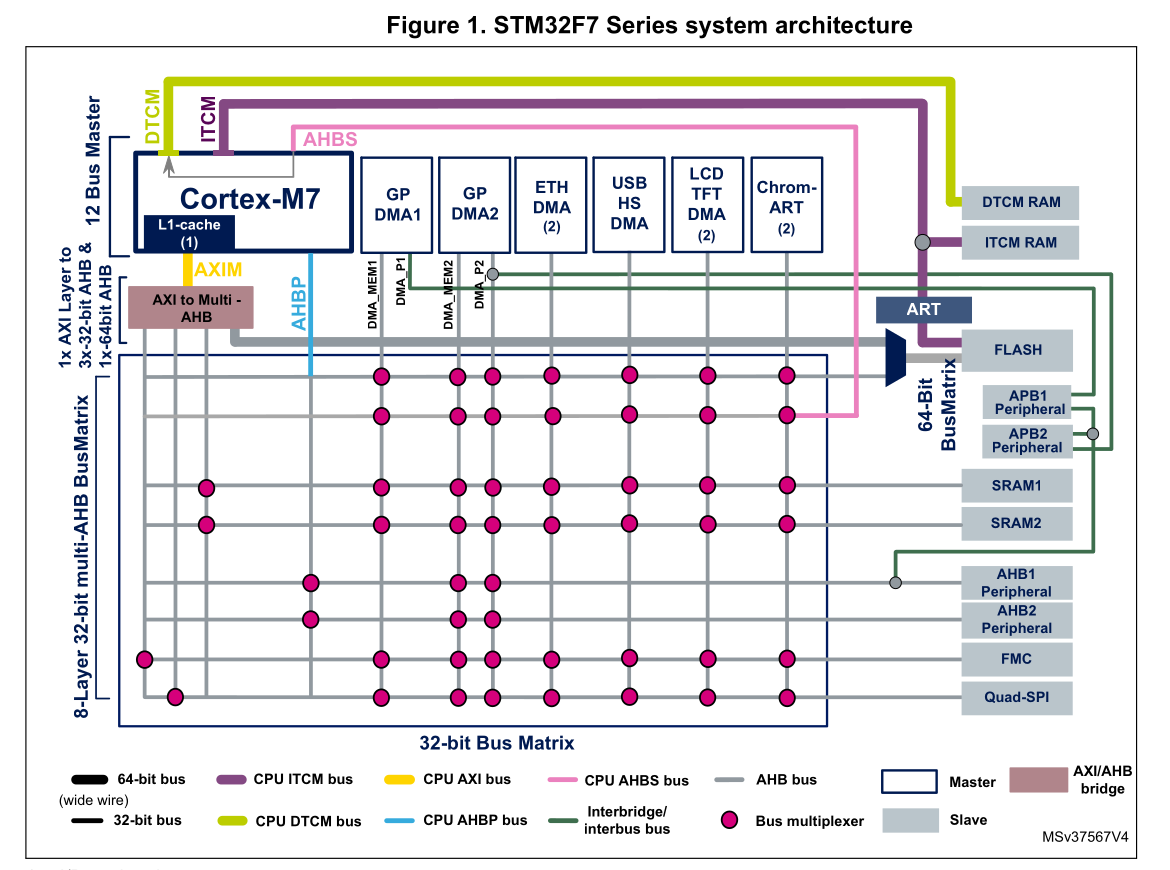
\includegraphics[width=1\textwidth]{assets/m7_system_arch}
    \caption{STM32F7 Systemarchitektur \cite[S. 9]{an4667}}
    \label{fig:m7_sys_arch}
\end{figure}

Aus der Matrix wird deutlich, dass für den Speicher zwischen SRAM und TCM-RAM
unterschieden wird. Der \ac{TCM} verfügt jeweils für Instruktionen und Daten
über einen dedizierten Kanal zum Prozessor und ist nicht cachefähig, bietet aber
als Besonderheit niedrigere Zugriffszeiten als SRAM. Während bei SRAM die
Zugriffszeit variieren kann (schnell aus dem Cache oder langsam aus dem
Speicher), ist die Zugriffszeit bei TCM konsistent und deterministisch. Dies
macht sie besonders geeignet für zeitkritische Routinen wie Interrupt-Handler
oder Echtzeitaufgaben. (\cite{arm_den0042})

Zusammenfassend lässt sich sagen, dass jeder normale, nicht gemeinsam genutzte
(non-shared) Speicherbereich gecacht werden kann, sofern er über das AXI-Bus
zugänglich ist \cite[S. 4]{an4839}~\cite[S. 7]{an4667}.

Aus der Tabelle für den internen Speicher wird deutlich, dass der Flash ab der
Adresse $0x0800 0000$ über das AXI-Bus angesprochen wird
(\ref{fig:internal_mem_table}). Diese Adresse ist auch im Linker-Skript
standardmäßig für den Flash festgelegt. Daher kann der I-Cache über den AXI-Bus
für den Flash genutzt werden, sofern der Boot-Pin sowie die assoziierten
\mintinline{text}|BOOT_ADDx| Option unverändert bleiben und die Firmware an die
Standardadresse geflasht wird \cite[S. 28]{stm32_datasheet}.

\begin{figure}[htb]
    \centering
    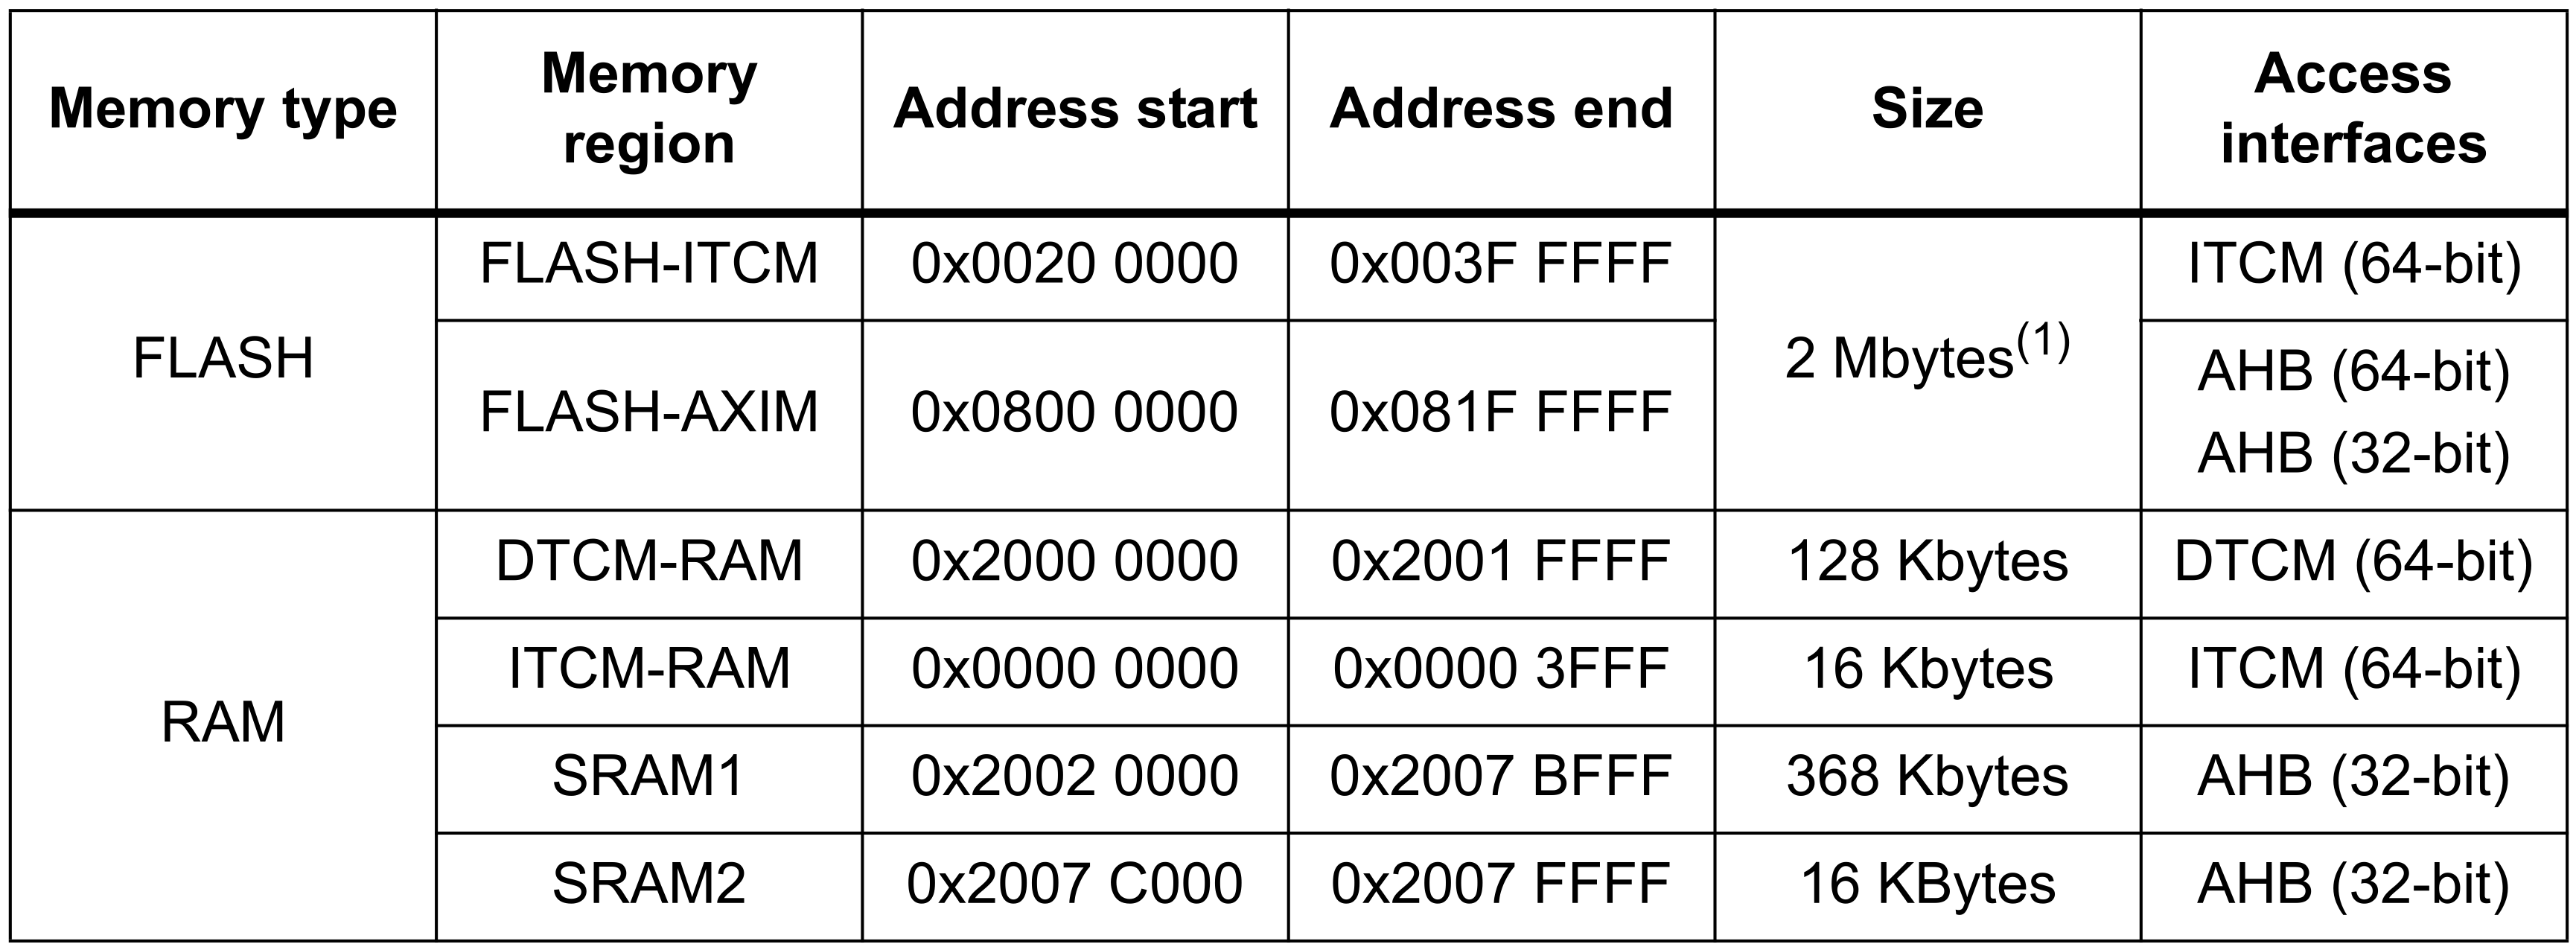
\includegraphics[width=1\textwidth]{assets/internal_mem_table}
    \caption{STM32F7 Speicheradressen \cite[S. 14]{an4667}}
    \label{fig:internal_mem_table}
\end{figure}

\begin{code}
\begin{minted}{c}
MEMORY
{
RAM (xrw)      : ORIGIN = 0x20000000, LENGTH = 512K
FLASH (rx)      : ORIGIN = 0x8000000, LENGTH = 2048K
}
\end{minted}
    \captionof{listing}{Definition Speicherbereich im Linker-Script für STM32F7}
\end{code}

Um Caches zu nutzen, bietet die STM-\ac{HAL} dedizierte Funktionsaufrufe in der
API an \cite[S. 4]{an4839}:

\begin{code}
\begin{minted}{c}
void SCB_EnableICache(void)
void SCB_EnableDCache(void)
void SCB_DisableICache(void)
void SCB_DisableDCache(void)
void SCB_InvalidateICache(void)
void SCB_InvalidateDCache(void)
void SCB_CleanDCache(void)
void SCB_CleanInvalidateDCache(void)
\end{minted}
    \captionof{listing}{Cache-Funktionen}
\end{code}

Bei einer Cache-Clean werden modifizierte Cache-Zeilen (Dirty Cache Lines), die
durch das Programm aktualisiert wurden, zurück in den Hauptspeicher geschrieben
\cite[S. 4]{an4839}. Dieser Vorgang wird gelegentlich auch als „flush”
bezeichnet. Eine Cache-Invalidierung markiert den Inhalt des Caches als
ungültig, sodass bei einem erneuten Zugriff auf dieselben Daten der Speicher neu
ausgelesen und der Cache aktualisiert werden muss.

Allerdings kann beim Aktivieren von Caches für Speicherbereiche, die vom
DMA-Controller genutzt werden, ein Problem der Cache-Kohärenz (Cache Coherency)
entstehen, da der Prozessor in diesem Fall nicht mehr der einzige Master ist,
der auf diese Speicherbereiche zugreift.

\subsubsection{Cache-Clean bei DMA} \label{sec:cache_clean}

Damit der DMA-Controller stets auf korrekte Daten zugreifen kann, ist eine
Cache-Clean nach jeder Modifikation der Daten erforderlich \cite[S. 6]{an4839}.
Ohne diesen Schritt würden die Änderungen nicht im SRAM widergespiegelt, und der
DMA-Controller würde weiterhin veraltete Daten verwenden.

\subsubsection{Cache-Invalidierung bei DMA}

Bei Daten, die aus dem Speicher gelesen werden, auf die auch der DMA-Controller
zugreift und modifiziert, muss vor jedem Lesevorgang eine Cache-Invalidierung
erfolgen \cite{embeddedexpert_cache}. Da der DMA-Controller die Daten jederzeit
ändern kann, sind die gecachten Daten per se ungültig und müssen immer durch
Aktualisierung ersetzt werden.

\subsection{Methode zur Echtzeitanalyse} \label{sec:dwt}

Um die Echtzeitanalyse der Steuerungssoftware durchzuführen, ist eine Methode
erforderlich, mit der beliebige Ausführungsabschnitte der Software flexibel,
präzise und threadsicher gemessen werden können. Da die Software multithreaded
ist, muss ebenfalls sichergestellt werden, dass die Messungen trotz preemptivem
Scheduling sowie Interrupts korrekt und zyklengetreu durchgeführt werden können.

Basierend auf den oben genannten Herausforderungen bietet die \ac{DWT} als eine
geeignete Lösung \cite{ARM_KA001499}. Die DWT ist ein Debug-Einheit in
Prozessoren inklusive ARMv7-M \cite{ARMv7_ref_man_dwt_about}, die das Profiling
mittels verschiedener Zähler unterstützen \cite{ARMv7_ref_man_dwt_profiling}.
Ein für diese Arbeit zentraler Teil der DWT ist der Zyklenzähler
\mintinline{c}|DWT_CYCCNT|, der bei jedem Takt inkrementiert wird, solange sich
der Prozessor nicht im Debug-Zustand befindet \cite{ARMv7_ref_man_dwt_cycle}.
Dadurch ermöglicht die DWT beispielsweise die Erfassung von Echtzeitaspekten mit
zyklengenauer Präzision under normaler Operation \cite{ARMv7_ref_man_dwt}.

\subsubsection{Beispiel: Segger SystemView}

Ein Beispiel hierfür ist Segger SystemView, ein Echtzeit-Analysewerkzeug, das
die DWT einsetzt, um Live-Code-Profiling auf eingebetteten Systemen
durchzuführen \cite{SEGGER_SystemView}.

Das Segger SystemView nutzt den DWT-Zyklenzähler, indem die Funktion \linebreak
\mintinline{c}|SEGGER_SYSVIEW_GET_TIMESTAMP()| für Cortex-M3/4/7-Prozessoren
einfach die hardkodierte Registeradresse des Zyklenzählers zurückgibt \cite[S.
65]{Segger_SystemView_manual}\cite{Arm_DWT_Programmers_Model}, anstatt die
interne Funktion \mintinline{c}|SEGGER_SYSVIEW_X_GetTimestamp()| aufzurufen.

\newpage

\section{Vorbereitung}

Die Vorbereitungsphase umfasst die Umstellung auf FreeRTOS und damit die
vollständige Ablösung von Micro-ROS. Der Datenaustausch wird intern über
FreeRTOS-Queues realisiert, während die Task-Synchronisation auf
Direct-Task-Notification anstatt von Semaphoren basiert. Zusätzlich wird die
Eingabe von Sollgeschwindigkeiten über UART mit CRC implementiert. Die
Aktivierung des Caches bildet den Abschluss dieser Vorbereitungen. Die Details
zu diesen Maßnahmen werden in den folgenden Abschnitten erläutert.

\subsection{Umstellung auf FreeRTOS}

\subsubsection{Geschwindigkeitsempfang über UART auf Mikrocontroller}

In der bisherigen Implementierung wurde der Geschwindigkeitssollwert vom
Host-System über ROS2 von dem Micro-ROS-Agent an den Client auf den MCU
übertragen. Um die Abhängigkeit von Micro-ROS komplett zu beseitigen, muss die
Übertragung und Interpretierung der Geschwindigkeitssollwerte manuell
implementiert werden.

Es wird zunächst ein einfacher Struct \mintinline{cpp}|Vel2d| definiert, um die
Geschwindigkeitswerte zu interpretieren, die vom Benutzer an den MCU gesendet
werden.

\begin{code}
\begin{minted}{cpp}
struct Vel2d {
  double x;
  double y;
  double omega;
};
\end{minted}
    \captionof{listing}{Definition der Struktur für die Sollgeschwindigkeit}
\end{code}

Darauf aufbauend wird eine weitere Struct \mintinline{cpp}|Vel2dFrame|
definiert, die als UART-Daten-Frame dient. Dieser enthält ein zusätzliches Feld
\mintinline{cpp}|crc| für die CRC-Überprüfung und eine Methode
\mintinline{cpp}|compare()|, die einen lokal kalkulierten CRC-Wert als Parameter
entgegennimmt, um diesen mit dem empfangenen zu vergleichen. Mit dem Attribut
\linebreak\mintinline{cpp}|__attribute__((packed))| wird verhindert, dass
zusätzliches Padding für die Speicherausrichtung dieses Typs eingefügt wird,
Damit die über UART empfangenen Bytes direkt als Objekt dieses Typs
interpretiert werden können.

\begin{code}
\begin{minted}{cpp}
struct Vel2dFrame {
  Vel2d vel;
  uint32_t crc;

  bool compare(uint32_t rhs) { return crc == rhs; }
} __attribute__((packed));

inline constexpr std::size_t VEL2D_FRAME_LEN = sizeof(Vel2dFrame);
\end{minted}
    \captionof{listing}{Definition der Data-Frame für die Sollgeschwindigkeit}
\end{code}

Für die Übertragung über UART kann die Setup-Funktion \linebreak
\mintinline{cpp}|HAL_UARTEx_ReceiveToIdle_IT()| aus der STM32-HAL-Bibliothek
verwendet werden, um die serialisierten Bytes eines Data-Frames zu empfangen.
Sie nimmt das UART-Handle, die Adresse eines Datenpuffers und dessen Größe
entgegen und empfängt die eingehenden Daten über Interrupts in diesen vorab
zugewiesenen Puffer.

Dies ist gepaart mit einer Interrupt-Callback
\mintinline{cpp}|HAL_UARTEx_RxEventCallback()|, die entweder ausgelöst wird,
wenn - wie der Name der UART-Setup-Funktion bereits andeutet - die UART-Leitung
feststellt, dass die Übertragung für eine bestimmte Zeit (abhängig von der
Baudrate) inaktiv war, oder wenn der Puffer für die Übertragung voll ist, was
darauf hinweist, dass der gesamte Inhalt des Puffers verarbeitet werden kann
\cite{HAL_UARTEx_ReceiveToIdle_IT}. Der zweite Parameter dieser
Interrupt-Callback gibt die Größe der in den Puffer geschriebenen Daten an
\cite{HAL_UARTEx_RxEventCallback}.

Mit diesem Setup kann die Software nun Bytes beispielsweise über UART direkt von
einem Linux-Host-Rechner empfangen, der mit dem MCU-Board verbunden ist.

\begin{code}
\begin{minted}{cpp}
// preallocated buffer with the exact size of a data frame
static uint8_t uart_rx_buf[VEL2D_FRAME_LEN];
volatile static uint16_t rx_len;

void HAL_UARTEx_RxEventCallback(UART_HandleTypeDef* huart, uint16_t size) {
  if (huart->Instance != huart3.Instance) return;

  rx_len = size;
  static BaseType_t xHigherPriorityTaskWoken;
  configASSERT(task_handle != NULL);
  vTaskNotifyGiveFromISR(task_handle, &xHigherPriorityTaskWoken);
  portYIELD_FROM_ISR(xHigherPriorityTaskWoken);

  // reset reception from UART
  HAL_UARTEx_ReceiveToIdle_IT(&huart3, uart_rx_buf, sizeof(uart_rx_buf));
}

// setup reception from UART in task init
HAL_UARTEx_ReceiveToIdle_IT(&huart3, uart_rx_buf, sizeof(uart_rx_buf));
\end{minted}
    \captionof{listing}{Nutzung STM32-HAL-API für den Datenempfang über UART via
    Interrupt}
\end{code}

Um die empfangenen Bytes zu parsen, ohne dies aber während der Ausführung der
Interrupt-Callback zu tun, wird ein eigenständiger FreeRTOS-Task erstellt.
Diesem Task wird von der Interrupt-Callback mittels
\mintinline{cpp}|vTaskNotifyGiveFromISR()|
signalisiert~\ref{sec:direct_task_notification} und die empfangenen Bytes werden
wieder in ein Data-Frame deserialisiert, um die Geschwindigkeit und die CRC zu
extrahieren.

Demnach kann dann eine CRC zur Kontrolle lokal aus den empfangenen
Geschwindigkeitswert berechnet werden und sie mit der empfangenen vergleichen.
Durch die Nutzung der dedizierten CRC-Peripherie ist die Berechnung
beispielsweise auf einem STM32-F37x-Gerät das 60-fache schneller, und verwendet
dabei nur 1,6\% der Taktzyklen im Vergleich zur Softwareberechnung \cite[S.
9]{AN4187}.

\begin{code}
\begin{minted}{cpp}
  while (true) {
    ulTaskNotifyTake(pdTRUE, portMAX_DELAY);

    len = rx_len;  // access atomic by default on ARM
    if (len != VEL2D_FRAME_LEN) {
      ULOG_ERROR("parsing velocity failed: insufficient bytes received");
      continue;
    }

    auto frame = *reinterpret_cast<const Vel2dFrame*>(uart_rx_buf);
    auto* vel_data = reinterpret_cast<uint8_t*>(&frame.vel);
    if (!frame.compare(HAL_CRC_Calculate(
            &hcrc, reinterpret_cast<uint32_t*>(vel_data), sizeof(frame.vel)))) {
      ULOG_ERROR("crc mismatch!");
      ++crc_err;
      continue;
    }

    frame.vel.x *= 1000;  // m to mm
    frame.vel.y *= 1000;  // m to mm

    xQueueSend(freertos::vel_sp_queue, &frame.vel, NO_BLOCK);
  }
\end{minted}
    \captionof{listing}{FreeRTOS-Task Dauerschleife}
\end{code}

\subsubsection{Geschwindigkeitsübertragung über UART auf Host}

Um den vom Benutzer festzulegenden Geschwindigkeitssollwert für den mobilen
Roboter zu übertragen, ist dem MCU-Board, auf dem die Steuerungssoftware läuft,
physisch per UART mit einem Linux-Host (einem Raspberry Pi 5) verbunden. Auf dem
Host wird das vorhandene ROS2-Paket \mintinline{text}|teleop_twist_keyboard|
verwendet, um Geschwindigkeitseingaben des Benutzers über die Tastatur zu
interpretieren. Um die Werten über UART zu senden, wird ein kleiner ROS2-Node
als Brücke erstellt, der den Micro-ROS-Agent ersetzt.

Dabei empfängt der Node über das ROS2-Framework die Geschwindigkeitssollwerte
und überträgt sie zusammen mit der im Konstruktur kalkulierten CRC an die
UART-Schnittstelle, die als abstrahierter serieller Port geöffnet ist.

\begin{code}
\begin{minted}{cpp}
class Vel2dBridge : public rclcpp::Node {
 public:
  Vel2dBridge() : Node{"vel2d_bridge"} {
    twist_sub_ = create_subscription<Twist>(
        "cmd_vel", 10, [this](Twist::UniquePtr twist) {
          auto frame =
              Vel2dFrame{{twist->linear.x, twist->linear.y, twist->angular.z}};

          if (!uart.send(frame.data())) {
            RCLCPP_ERROR(this->get_logger(), "write failed");
            return;
          }
          RCLCPP_INFO(this->get_logger(), "sending [%f, %f, %f], crc: %u",
                      frame.vel.x, frame.vel.y, frame.vel.omega, frame.crc);
        });
  }

 private:
  rclcpp::Subscription<Twist>::SharedPtr twist_sub_;
  SerialPort<VEL2D_FRAME_LEN> uart =
      SerialPort<VEL2D_FRAME_LEN>(DEFAULT_PORT, B115200);
};
\end{minted}
    \captionof{listing}{ROS2-Node Implementierung für
    Geschwindigkeitsübertragung}
\end{code}

Die CRC-Berechnung auf dem Host erfolgt mithilfe einer C++-Bibliothek von Daniel
Bahr \cite{CRCpp}. Der Algorithmus \mintinline{cpp}|CRC::CRC_32_MPEG2()|
entspricht demjenigen, der von der CRC-Peripherie des STM32-Boards verwendet
wird.

\begin{code}
\begin{minted}{cpp}
Vel2dFrame::Vel2dFrame(Vel2d vel)
    : vel{std::move(vel)},
      crc{CRC::Calculate(&vel, sizeof(vel), CRC::CRC_32_MPEG2())} {}
\end{minted}
    \captionof{listing}{CRC-Berechnung im Konstruktur}
\end{code}

Mithilfe dieser Implementierungen werden die Übertragung der
Geschwindigkeitssollwerte vom Host und deren Empfang auf dem MCU ermöglicht.
Dadurch, dass der Empfang detektiert, dass keine weiteren Bytes übertragen
werden, und ebenso durch die Überprüfung der CRC, werden unvollständige oder
fehlerhafte Bytes erkannt und verworfen, ohne den Programmablauf zu blockieren.

\subsubsection{Steuerungskomponenten als FreeRTOS-Task}

Analog zur Implementierung basierend auf Micro-ROS, bei der alle logischen
Komponenten als Single-Threaded-Executor abstrahiert werden, sind diese
Komponenten in FreeRTOS ebenfalls als eigenständige Tasks implementiert. Der
Fokus liegt hierbei darauf, den grundlegenden Datenaustausch in Form einer
Publisher-Subscriber-Architektur mittels Queues zu realisieren. Dadurch müssen
die Daten nicht mehr durch Semaphoren oder Mutexe geschützt werden, welche in
FreeRTOS auch nur mittels Queue-Objekte abstrahiert werden.

Zunächst wird ein eigenständiger Task zur Abfrage und Übertragung der
Encoderwerte erstellt, die von der Hardware bzw. der Hardwareabstraktion durch
Timer bereitgestellt werden, damit die anderen Tasks bei jeder Iteration auf
einheitliche Encoderwerte zugreifen können.

\begin{code}
\begin{minted}{cpp}
static void task_impl(void*) {
  constexpr TickType_t NO_BLOCK = 0;
  TickType_t xLastWakeTime = xTaskGetTickCount();
  const TickType_t xFrequency = pdMS_TO_TICKS(WHEEL_CTRL_PERIOD_MS.count());

  while (true) {
    auto enc_delta = FourWheelData(hal_encoder_delta_rad());

    xQueueSend(freertos::enc_delta_wheel_ctrl_queue, &enc_delta, NO_BLOCK);
    xQueueOverwrite(freertos::enc_delta_odom_queue, &enc_delta);

    vTaskDelayUntil(&xLastWakeTime, xFrequency);
  }
}
\end{minted}
    \captionof{listing}{FreeRTOS-Task für Encoderwertabfrage und -übertragung}
\end{code}


Der Empfänger-Task welchen mit \mintinline{cpp}|xQueueSend()| addressiert wird,
läuft mit einer höhreren Frequenz, sodass er die Daten immer sofort verarbeitet
und auf neue Daten wartet. Im Gegensatz dazu ist
\mintinline{cpp}|xQueueOverwrite()| eine spezielle Funktion, die ausschließlich
für Queues mit einer maximalen Kapazität von einem Objekt vorgesehen ist. Sie
überschreibt das vorhandene Objekt in der Queue, falls es existiert. In diesem
Kontext ist dies jedoch irrelevant, da der zugehörige Empfänger-Task, der mit
der gleichen Frequenz wie der Encoderwert-Task läuft, die Daten synchron
verarbeitet. Dennoch dient die Überschreibbarkeit als zusätzliche
Sicherheitsmaßnahme für den Fall, dass unerwartete Szenarien auftreten.

Darauf basierend kann die Kommunikation als Matrix wie folgt illustriert werden:

\begin{table}[h!]
\centering
\small
\setlength{\tabcolsep}{4pt} % Reduce column padding
\begin{tabular}{|c|c|c|c|}
\hline
    \diagbox{Sendertask}{Empfängertask} & \textbf{Odometrie} & \textbf{Drehzahlregelung} & \textbf{Posenregelung} \\ \hline
\textbf{Encoderwerte}               & $\rightarrow$             & $\rightarrow$       &               \\ \hline
\textbf{Geschwindigkeitssollwert}   &                           &                     & $\rightarrow$ \\ \hline
\textbf{Odometrie}                  & \cellcolor{gray!20}       &                     & $\rightarrow$ \\ \hline
\textbf{Drehzahlregelung}           &                           & \cellcolor{gray!20} & $\rightarrow$ \\ \hline
\end{tabular}
\caption{Kommunikationskanal-Matrix}
% \label{tab:kommunikationsmatrix}
\end{table}

Die Kanäle werden dementsprechend durch Queue-Objekte repräsentiert.

\begin{code}
\begin{minted}{cpp}
extern QueueHandle_t enc_delta_odom_queue;
extern QueueHandle_t enc_delta_wheel_ctrl_queue;
extern QueueHandle_t vel_sp_queue;
extern QueueHandle_t odom_queue;
extern QueueHandle_t vel_wheel_queue;
\end{minted}
    \captionof{listing}{Queue-Objekte in FreeRTOS}
\end{code}

Die grundlegende Implementierung der jeweiligen Steuerungstasks bleibt
größententeils von der Micro-ROS-Struktur erhalten. Die Initialisierung der
jeweiligen Steuerungstasks erfolgt in \mintinline{cpp}|freertos::init()|:

\begin{code}
\begin{minted}{cpp}
void init() {
  hal_init();
  queues_init();
  task_hal_fetch_init();
  task_vel_recv_init();
  task_pose_ctrl_init();
  task_wheel_ctrl_init();
  task_odom_init();
}
\end{minted}
    \captionof{listing}{Initialisierung von FreeRTOS-Tasks}
\end{code}

Eine üblicher Ansatz in einem FreeRTOS-System, um unter anderem sowohl den
Speicherverbrauch zu optimieren als auch die Programmdeterminiertheit zu
verbessern, besteht darin, die Erstellung der FreeRTOS-Objekte statisch
durchzuführen.

Um diese zu realisieren, wird im Makefile ein Macro
\mintinline{text}|-DFREERTOS_STATIC_INIT| definiert, das zur
Übersetzungszeit festlegt, ob die Objekte dynamisch innerhalb der FreeRTOS-API
oder statisch mit benutzerdefinierten Speicherorten zugewiesen werden sollen.

Für einen Task, der dynamisch allokiert wird, ist der Funktionsaufruf so einfach
wie der folgende:

\begin{code}
\begin{minted}{cpp}
xTaskCreate(task_impl, "hal_fetch", STACK_SIZE,
            NULL, osPriorityNormal, &task_handle);
\end{minted}
    \captionof{listing}{Dymanische Allokation eines FreeRTOS-Tasks}
\end{code}

Wenn ein Task statisch allokiert werden soll, muss der Benutzer manuell jeweils
einen Speicherpuffer für den Task-Stack und für den Task selbst deklarieren und
an die API übergeben.

\begin{code}
\begin{minted}{cpp}
static StackType_t taskStack[STACK_SIZE];
static StaticTask_t taskBuffer;
task_handle = xTaskCreateStatic(
                    task_impl, "hal_fetch", STACK_SIZE, NULL, osPriorityNormal,
                    taskStack, &taskBuffer);
\end{minted}
    \captionof{listing}{Dymanische Allokation eines FreeRTOS-Tasks}
\end{code}

Analog dazu muss der Benutzer für die statische Allokation einer Queue auch
jeweils einen Speicherpuffer mit der maximalen Kapazität für die Queue und für
die Queue selbst deklarieren:

\begin{code}
\begin{minted}{cpp}
 constexpr size_t QUEUE_SIZE = 10;
 static FourWheelData buf[QUEUE_SIZE];
 static StaticQueue_t static_queue;
 return xQueueCreateStatic(QUEUE_SIZE, sizeof(*buf),
                           reinterpret_cast<uint8_t*>(buf), &static_queue);
\end{minted}
    \captionof{listing}{Dymanische Allokation einer FreeRTOS-Queue}
\end{code}

Damit schließt der Abschnitt zur Umstellung auf FreeRTOS. Der Code für die
MCU-Software sowie für den ROS2-Node auf dem Host ist im
Repository~\cite{mecarover_freertos_profiling} verfügbar.

\newpage

\subsection{Aktivierung von Caches}

TODO

\newpage

\section{Abschluss}

Am Anfang wurde die Robotersteuerungssoftware von Micro-ROS auf FreeRTOS
umgestellt. Anschließend wurden eine Multi-Producer-Senke sowie ein Verfahren
entwickelt, das Echtzeitinformationen über die Steuerungssoftware ausgeben kann.
Abschließend wurde die Echtzeitfähigkeit basierend auf die Echtzeitinformationen
analysiert.

\subsection{Fazit}

Es lässt sich schlussfolgern, dass die Steuerungssoftware zwar durch Integration
von Micro-ROS funktionsreicher und folglich mit einer Vielzahl von
ROS-Komponenten kompatibel wird, dies allerdings mit erheblichem Overhead
erkauft wird. Bei begrenztem Speicher oder Rechenleistung bleibt FreeRTOS mit
seinem schlanken Kernel und den threadsicheren Queue-Implementierungen weiterhin
eine geeignete Wahl gegenüber komplexeren RTOS-Lösungen -- besonders wenn harte
Echtzeitfähigkeit im Vordergrund steht.

Darüber hinaus wurde gezeigt, dass sich die Softwareleistung durch L1-Caches
deutlich verbessern lässt, was für leistungskritische Software entscheidend ist.

\subsection{Ausblick}

Für zukünftige Arbeiten könnte die Multi-Producer-Senke so weiterentwickelt
werden, dass sie atomare Schreiboperationen auf 4-Byte-/32-Bit-Ebene
unterstützt. Dadurch könnten die Echtzeit-Daten nicht mehr im menschenlesbaren
Format, sondern maschinenlesbar und komprimiert als 4-Byte-Dateneinheit
ausgegeben werden.

Dies würde den Zwischenpuffer für die Echtzeitanalyse überflüssig machen, da die
durch Kontextwelchsel/Interrupt generierten Daten direkt atomar in die Senke
geschrieben werden könnten. Dazu müsste ein Parser auf dem Host-System
entwickelt werden, der idealerweise auch die Visualisierung sowie Analyse der
Daten parallel in Echtzeit ermöglicht.

\newpage

% einfacher Zeilenabstand
\singlespacing
% Literaturliste soll im Inhaltsverzeichnis auftauchen
\newpage
\phantomsection
\addcontentsline{toc}{section}{Literaturverzeichnis}
% Literaturverzeichnis anzeigen
\renewcommand\refname{Literaturverzeichnis}
\bibliography{Hauptdatei}

%% Index soll Stichwortverzeichnis heissen
% \newpage
% % Stichwortverzeichnis soll im Inhaltsverzeichnis auftauchen
% \addcontentsline{toc}{section}{Stichwortverzeichnis}
% \renewcommand{\indexname}{Stichwortverzeichnis}
% % Stichwortverzeichnis endgültig anzeigen
% \printindex

% \onehalfspacing
% % evtl. Anhang
% \newpage
% \phantomsection
% \addcontentsline{toc}{section}{Anhang}
% \fancyhead[L]{Anhang} %Kopfzeile links
% \input{anhang}

\newpage
% \includepdf[pages=1, fitpaper=true]{eigenstaendigkeitserklaehrung.pdf}

% \fancyhead[L]{Eigenständigkeitserklährung} %Kopfzeile links
% \input{eigenstaendigkeitserklaehrung} % deleted 

\end{document}
